\chapter{Implementation}
\label{chp:implementation}

% %
% HEADER
% %
In this Section we show the reference architecture of the auto-scaling service.

The auto-scaling service provides Kubernetes with the best replication degree for its containers, determined by the adopted reinforcement learning technique applied to the current state of the cluster.
%
The service is realized by the following three main components, interacting via REST interfaces:

\begin{itemize}
	
	\item \texttt{ClusterMonitor} collects cluster performance metrics. Exposes a REST interface to retrieve these metrics.
	%
	In a usual Kubernetes cluster, this component is realized by the Heapster master.
	
	\item \texttt{Orchestrator} responsible for container orchestration. This component scales in/out its containers accordingly with the \texttt{ScalingAction} provided by \texttt{ScalerAI}. It pulls the \texttt{ScalerAI} at fixed time interval to retrieve the action with respect to the current cluster state. It identifies itself to the \texttt{ScalerAPI} by a alphanumeric \texttt{APIToken}.
	%
	In a usual Kubernetes cluster, this component is realized by the Kubernetes leading master.
	
	\item \texttt{ScalerAI} responsible to determine the best \texttt{ScalingAction} with respect to the current \texttt{ClusterState}.
	%
	It exposes a REST interface through which the \texttt{Orchestrator} asks it to produce a new \texttt{ScalingAction}.
	%
	When the component is asked to produce a new \texttt{ScalingAction}, the \texttt{StateManager} collects cluster metrics from the \texttt{ClusterMonitor} and aggregates them into a new \texttt{ClusterState}.
	%
	The latter is then submitted as input to the \texttt{RLEngine} that executes a new reinforcement learning iteration, thus producing a new \texttt{ScalingAction} to be returned to the \texttt{Orchestrator}.
	
\end{itemize}

In Figure~\ref{fig:implementation-architecture} we show the reference high-level architecture for the auto-scaling service, represented as a UML component diagram.

\begin{figure}	
	\label{fig:implementation-architecture}
	\centering
	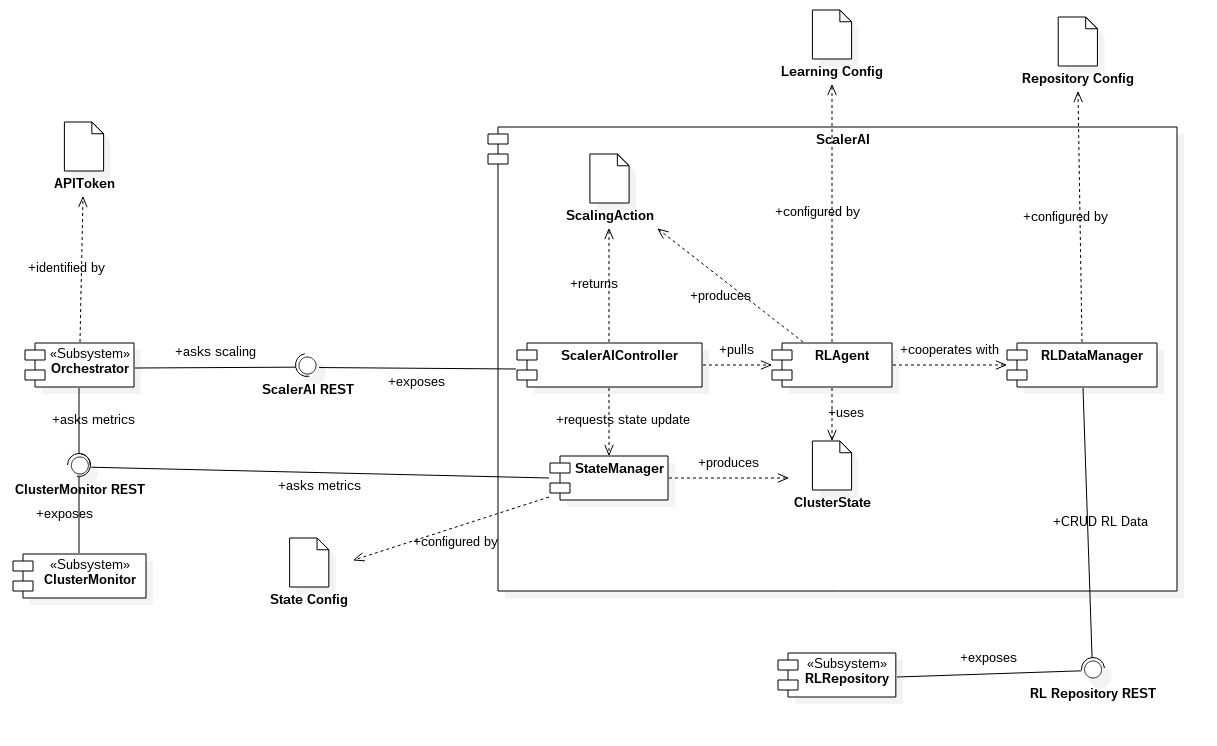
\includegraphics[width=.85\columnwidth]{implementation-architecture}
	\caption{The Architecture}
\end{figure}


% %
% REST API
% %
\section{REST Interfaces}
\label{sec:implementation-rest-interfaces}

In this section we detail the REST API exposed by \texttt{ScalerAI} to provide \texttt{Orchestrator} with \texttt{ScalingAction}. Furthermore we detail the REST calls executed by \texttt{ScalerAI} on \texttt{ClusterMonitor} to gather the performance metrics.



